\documentclass[12pt]{article}

\usepackage[utf8]{inputenc}
\usepackage[english]{babel}

\usepackage{fullpage}
\usepackage{microtype}

\usepackage{tikz}
\usepackage[colorlinks=true, linkcolor=red, urlcolor=blue]{hyperref}

\usepackage{amsfonts, amsmath, amsthm}
\newtheorem{theorem}{Theorem}
\newtheorem{definition}{Definition}
\newtheorem{lemma}{Lemma}
\newtheorem{corollary}{Corollary}
\newtheorem{conjecture}{Conjecture}
\newtheorem{example}{Example}

\newcommand{\abs}[1]{\lvert #1 \rvert}

\newcommand{\Z}{\mathbb{Z}}
\newcommand{\R}{\mathbb{R}}
\newcommand{\N}{\mathbb{N}}
\newcommand{\Q}{\mathbb{Q}}

\begin{document}
	\title{Eigenvalues of Square \textit{Lights Out} Games}
	\author{William Boyles}
	\maketitle
	
	\section{Definitions}
	\begin{definition}\label{def:matrix}
		The $n$th \textit{Lights Out} matrix with diagonal $k$ is the $n^2 \times n^2$
		block matrix of the form
		\begin{equation*}
		M_{n,k} = \begin{bmatrix}
		D_{n,k} & I_n & O_n & O_n & O_n & \ldots & O_n \\
		I_n & D_{n,k} & I_n & O_n & O_n & \ldots & O_n \\
		O_n & I_n & D_{n,k} & I_n & O_n & \ldots & O_n \\
		\vdots & \ddots & \ddots & \ddots & \ddots & \ddots & \vdots \\
		O_n & \ldots & O_n & I_n & D_{n,k} & I_n & O_n \\
		O_n & \ldots & O_n & O_n & I_n & D_{n,k} & I_n \\
		O_n & \ldots & O_n & O_n & O_n & I_n & D_{n,k}
		\end{bmatrix}
		\end{equation*}
		where $I_n$ is the $n \times n$ identity matrix, $O_n$ is the $n \times n$ zero
		matrix, and $D_{n,k}$ is the tridiagonal $n \times n$ matrix with $k$ along the
		main diagonal, $1$ above and below the main diagonal, and $0$ elsewhere.
		\begin{equation*}
		D_{n,k} = \begin{bmatrix}
		k & 1 & 0 & 0 & 0 & \ldots & 0 \\
		1 & k & 1 & 0 & 0 & \ldots & 0 \\
		0 & 1 & k & 1 & 0 & \ldots & 0 \\
		\vdots & \ddots & \ddots & \ddots & \ddots & \ddots & \vdots \\
		0 & \ldots & 0 & 1 & k & 1 & 0 \\
		0 & \ldots & 0 & 0 & 1 & k & 1 \\
		0 & \ldots & 0 & 0 & 0 & 1 & k
		\end{bmatrix}.
		\end{equation*}
		$k \in \N$.
	\end{definition}
	
	\begin{definition}\label{def:innerprod}
		The inner product of two vectors in $\Z_{2}^{n^2}$ is the result of their
		standard inner product in $\R^{n^2}$ $\mod 2$.
	\end{definition}
	\begin{definition}\label{def:converted}
		A vector $\vec{v}$ in $\R^{n^2}$ is convertible to a vector in $\Z_{2}^{n^2}$
		if there exists a real, non-zero constant $c$ such that $c\vec{v}$ has all
		integer components. 
		The converted vector is $\vec{v_2} = c\vec{v} \mod 2$.
	\end{definition}
	
	\section{Some Lemmas}
	Below are some lemmas that will be useful in proving our main theorems and
	their corollaries. They are in this section rather than immediately before where
	they are first applied because they are applicable outside the specific context
	of \textit{Lights Out}.
	\begin{lemma}\label{lem:convert}
		All eigenvectors with rational eigenvalues of a matrix with all rational
		entries are convertible.
	\end{lemma}
	\begin{proof}
		Let $A$ be a square matrix with all rational entries. 
		Let $\lambda$ be an eigenvalue of $A$.
		Consider the process of finding eigenvectors from a rational eigenvalue. 
		One would do elementary row operations on the homogeneous system $(A-\lambda
		I)\vec{v} = \vec{0}$. 
		Since $\lambda$ is rational, all of the entries in $A$ are also rational, and
		elementary row operations do not introduce irrational numbers, then the
		resultant vector has all rational entries. 
		Let
		\begin{equation*}
		\vec{v} = \left(\frac{p_1}{q_1}, \frac{p_2}{q_2}, \ldots,
		\frac{p_{n^2}}{q_{n^2}}\right)^\text{T}
		\end{equation*}
		be the resultant eigenvector, where each $p_i / q_i$ is a fraction of integers
		in least terms.
		Then multiplying $\vec{v}$ by $k = \text{lcm}{\left(q_1, q_2, \ldots,
			q_{n^2}\right)}$ gives a vector with all integer components, so $\vec{v}$ is
		convertible.
	\end{proof}
	Within the context of \textit{Lights Out}, this means all eigenvectors of
	$M_{n,k}$ with rational eigenvalues are convertible.
	Eigenvectors with irrational eigenvalues may still be convertible if the ratio
	of any two components of the eigenvector is rational.
	
	%	\begin{lemma}\label{lem:eigspacesize}
	%		Let $d$ be the dimension of any eigenspace $V_\lambda \subseteq \Z_2^{n^2}$.
	%Then the number of vectors in $V_\lambda$ is $2^d$.
	%	\end{lemma}
	%	\begin{proof}
	%		Let $B = \left\{\vec{b_1}, \vec{b_2}, \ldots, \vec{b_d}\right\} \subseteq
	%V_\lambda$ be a basis for $V_{\lambda}$.
	%		Then any vector $\vec{v} \in V_\lambda$ is a unique linear combination of
	%vectors in $B$.
	%		\begin{equation*}
	%			\vec{v} = a_1\vec{b_1} + a_2\vec{b_2} + \ldots + a_d\vec{b_d},
	%\hspace*{12pt} a_1, a_2, \ldots a_d \in \Z_2.
	%		\end{equation*}
	%		Since each $a_i$ is a binary integer, every vector in $V_\lambda$ can be
	%uniquely encoded as a binary string of length $d$: $s = s_1s_2\ldots s_d$,
	%where $s_i = ``a_i"$.
	%		There are $2^d$ unique binary strings of length $d$ and thus $2^d$ unique
	%vectors in $V_\lambda$.
	%	\end{proof}
	
	\begin{lemma}\label{lem:identeigvals}
		If $\lambda$ is an eigenvalue of a matrix $A$, then $\lambda - c$ is an
		eigenvalue of $B = A - cI$.
	\end{lemma}
	\begin{proof}
		Let $\lambda$ be an eigenvalue of $A$ with corresponding eigenvector
		$\vec{v}$. 
		Then
		\begin{equation*}
		B\vec{v} = (A-cI)\vec{v} = A\vec{v} - cI\vec{v} = \lambda\vec{v} - c\vec{v} =
		\left(\lambda-c\right)\vec{v}.
		\end{equation*}
		Thus, $\lambda - c$ is an eigenvalue of $B$ with eigenvector $\vec{v}$.
	\end{proof}
	
	%	\begin{lemma}[\href{https://en.wikipedia.org/wiki/Niven\%27s_theorem}{Niven's
	%Theorem}]\label{lem:nivens}
	%		For rational values of $\theta$ in degrees, the only rational values of
	%$\cos{\theta}$ are $0$, $\pm 1/2$, and $\pm 1$.
	%	\end{lemma}
	
	\begin{lemma}\label{lem:cos_sum1_nosol}
		Let $p$ and $q$ be rational numbers where $0 < p < q < 1$. Then there are no
		solutions to
		\begin{equation*}
		\cos{(\pi p)} + cos{(\pi q)} = 1.
		\end{equation*}
	\end{lemma}
	\begin{proof}
		Professor Jason Bell at the University of Waterloo proved in
		\href{https://www.reddit.com/r/math/comments/gsiqu8/conjecture_about_rational_angles/}{this}
		Reddit thread that for any rational number $C$ where
		\begin{equation*}
		\cos{(\pi p)} + cos{(\pi q)} = C,
		\end{equation*}
		that $N$, the common denominator of $p$ and $q$, is such that $\phi(N) < 8 /
		\abs{C}$ where $\phi$ is Euler's totient function. 
		%		He also mentions that we can loosely bound $N$ by $128 / C^2$.
		Taking this bound, I have checked via computer program that the only solution
		for $C = 1$ is
		\begin{equation*}
		\cos{\left(\frac{\pi}{3}\right)} + \cos{\left(\frac{\pi}{3}\right)} = 1.
		\end{equation*}
		Since this would make $p = q = 1/3$, and $p < q$, so there are indeed no
		solutions.
	\end{proof}
	We can apply the same techniques to show that for $C=-1$, the only solutions (allowing $p=q$) are $(p,q) = (2/3,2/3)$; for $C=1/2$, the only solutions are $(p,q) = (1/3,
	1/2)$ and $(1/5, 3/5)$; for $C=-1/2$, the only solutions are $(p,q) = (1/2,
	2/3)$ and $(2/5, 4/5)$.
	What's curious is that these solutions and the one given in lemma
	\ref{lem:cos_sum1_nosol} appear to be the only solutions, as conjectured in
	conjecture \ref{conj:cos_rationals}.
	
	\section{Normal \textit{Lights Out}: $k=1$}
	We will start by looking at the traditional \textit{Lights Out} game ($k=1$)
	and then generalize the results to all $k \in \N$.
	$M_{n,k}$ models the effect of clicking some of the $n^2$ buttons on an $n
	\times n$ \textit{Lights Out} board. 
	In the on or off context of \textit{Lights Out} lights, it is a endomorphism
	over $\Z_2^{n^2}$, but we can still analyze it as a endomorphism over
	$\R^{n^2}$. 
	For example, since $M_n$ is real and symmetric, all of its $n^2$ eigenvalues
	and the components of its eigenvectors are real. 
	Since the components of all vectors in $\Z_2^{n^2}$ are either $0$ or $1$, any
	eigenvectors of $M_{n,k}$ in $\Z_2^{n^2}$ would have an eigenvalue of $0$ or
	$1$. 
	These are the most important eigenpairs in the context of \textit{Lights Out}.
	
	\begin{lemma}\label{lem:k1eigvals}
		The eigenvalues of $D_{n,1}$ are
		\begin{equation*}
		\lambda_i = 1 + 2\cos{\left(\frac{i}{n+1}\pi\right)}, \hspace{12pt} 1 \leq i
		\leq n.
		\end{equation*}
	\end{lemma}
	
	\begin{proof}
		$p_n$, the characteristic polynomial of $D_{n,1}$ satisfies the recurrence
		relation
		\begin{equation*}
		p_n = \begin{cases}
		1 & n = 0 \\
		1-\lambda & n = 1 \\
		(1-\lambda)p_{n-1} - p_{n-2} & n \geq 2
		\end{cases}.
		\end{equation*}
		Letting $2x = 1-\lambda$, our recurrence relation becomes the definition of a
		Chebyshev polynomial of the second kind, $U_n(x)$. It's well-know that the roots
		of $U_n(x)$ are
		\begin{equation*}
		x_i = \cos{\left(\frac{i}{n+1}\pi\right)}, \hspace{12pt} 1 \leq i \leq n.
		\end{equation*}
		Since $\lambda = 1-2x$, we see that the roots of the characteristic polynomial
		of $D_n$ are
		\begin{equation*}
		\lambda_i = 1-2\cos{\left(\frac{i\pi}{n+1}\right)}, \hspace{12pt} 1 \leq i
		\leq n.
		\end{equation*}
		Since
		\begin{equation*}
		1 - 2\cos{\left(\frac{i\pi}{n+1}\right)} = 1 +
		2\cos{\left(\frac{n-i+1}{n+1}\pi\right)},
		\end{equation*}
		and $n-i+1$ has the same bounds as $i$, so we can write the eigenvalues as
		\begin{equation*}
		\lambda_i = 1 + 2\cos{\left(\frac{i}{n+1}\pi\right)}, \hspace{12pt} 1 \leq i
		\leq n.
		\end{equation*}
	\end{proof}
	
	\begin{theorem}\label{thm:k1eigvals}
		The eigenvalues of $M_{n,1}$ are are given by
		\begin{equation*}
		\lambda_{i,j} =
		\left(1+2\cos{\left(\frac{i}{n+1}\pi\right)}\right)+\left(2\cos{\left(\frac{j}{n+1}\pi\right)}\right),
		\hspace{12pt} 1 \leq i,j \leq n.
		\end{equation*}
	\end{theorem}
	\begin{proof}
		Since $M_{n,1}$ is a block matrix with similar structure to $D_{n,1}$, we can
		write it as a Kronecker product.
		\begin{equation*}
		M_{n,1} = D_{n,1} \otimes I_n + I_n \otimes (D_{n,1} - I_n).
		\end{equation*}
		
		In this case, Kronecker products have the property that the eigenvalues of
		$M_n$ are the sums of pairs of eigenvalues of $D_{n,1}$ and $D_{n,1} - I_n$. 
		By lemma \ref{lem:identeigvals} and lemma \ref{lem:k1eigvals}, we get that the
		eigenvalues of $M_{n,1}$ are
		\begin{equation*}
		\lambda_{i,j} =
		\left(1+2\cos{\left(\frac{i}{n+1}\pi\right)}\right)+\left(2\cos{\left(\frac{j}{n+1}\pi\right)}\right),
		\hspace{12pt} 1 \leq i,j \leq n.
		\end{equation*}
	\end{proof}
	
	\section{Generalization: $k \in \N$}
	We are now ready to generalize theorem \ref{thm:k1eigvals} and make some
	interesting corollaries.
	\begin{theorem}\label{thm:kanyeigvals}
		The eigenvalues of $M_{n,k}$ are given by
		\begin{equation*}
		\lambda_{i,j} =
		\left(k+2\cos{\left(\frac{i}{n+1}\pi\right)}\right)+\left(2\cos{\left(\frac{j}{n+1}\pi\right)}\right),
		\hspace{12pt} 1 \leq i,j \leq n.
		\end{equation*}
	\end{theorem}
	\begin{proof}
		\begin{equation*}
		M_{n,k} = M_{n,1} + (k-1)I.
		\end{equation*}
		Applying lemma \ref{lem:identeigvals} to the results of theorem
		\ref{thm:k1eigvals}, we get the eigenvalues as
		\begin{equation}\label{eq:kmanyeigvals}
		\lambda_{i,j} =
		\left(k+2\cos{\left(\frac{i}{n+1}\pi\right)}\right)+\left(2\cos{\left(\frac{j}{n+1}\pi\right)}\right),
		\hspace{12pt} 1 \leq i,j \leq n.
		\end{equation}
	\end{proof}
	
	We will focus on integer eigenvalues.
	Our goal as we work through these corollaries is to understand the structure
	and symmetries of the eigenvalues to the point where we can give a full
	description of where and under what conditions integer eigenvalues occur.
	
	\begin{corollary}
		\begin{equation*}
		\lambda_{i,j} = \lambda_{j,i}.
		\end{equation*}
	\end{corollary}
	\begin{proof}\label{cor:majorsymmetry}
		\begin{align*}
		\lambda_{i,j} &= k + 2\cos{\left(\frac{i}{n+1}\pi\right)} +
		2\cos{\left(\frac{j}{n+1}\pi\right)} \\
		&= k + 2\cos{\left(\frac{j}{n+1}\pi\right)} +
		2\cos{\left(\frac{i}{n+1}\pi\right)} \\
		&= \lambda_{j,i}.
		\end{align*}
	\end{proof}
	Although this corollary is certainly the simplest, it describes an important
	symmetry in the eigenvalues of $M_{n,k}$ that we will use repeatedly to prove
	more interesting results.
	If the eigenvalues of $M_{n,k}$ were laid out on an $n \times n$ matrix
	according to their $i$ and $j$ values -- $(i,j)=(1,1)$ in the upper left and
	$(n,n)$ in the bottom right -- then this result tells us that the matrix is real
	and symmetric about the major diagonal.
	
	\begin{corollary}\label{cor:charpolymultiplicity}
		The characteristic polynomial of $M_{n,k}$ has a root of multiplicity $n$ at
		$\lambda = k$.
	\end{corollary}
	\begin{proof}
		Rearranging equation \eqref{eq:kmanyeigvals} to use multiplication instead of
		addition,
		\begin{equation}\label{eq:kmanyeigvals_mult}
			\cos{\left(\frac{i+j}{n+1}\cdot\frac{\pi}{2}\right)}\cos{\left(\frac{i-j}{n+1}\cdot\frac{\pi}{2}\right)} = \frac{k-\lambda_{i,j}}{4}, \hspace{12pt} 1\leq i,j \leq n.
		\end{equation}
		Substituting $\lambda_{i,j} = k$,
		\begin{align*}	
			\cos{\left(\frac{i+j}{n+1}\cdot\frac{\pi}{2}\right)}\cos{\left(\frac{i-j}{n+1}\cdot\frac{\pi}{2}\right)}
			= 0&, \hspace{12pt} 1\leq i,j \leq n \\
			\implies \cos{\left(\frac{i+j}{n+1}\cdot\frac{\pi}{2}\right)} = 0&,
			\hspace{12pt} 1\leq i,j \leq n
		\end{align*}
		because the second $\cos$ term is never $0$ for our bounds on $i$ and $j$.
		\begin{align*}
		\implies i+j = n+1, \hspace{12pt} 1\leq i,j \leq n
		\end{align*}
		giving exactly $n$ solutions.
	\end{proof}
	We've now added some more detail to our matrix of eigenvalues.
	Along the minor diagonal, from bottom left to top right, all eigenvalues are
	$k$.
	This hints at some sort of symmetry about the minor diagonal, which we will
	address next.
	
	\begin{corollary}\label{cor:sum2k}
		\begin{equation*}
		\lambda_{i,j} + \lambda_{n-i+1,n-j+1} = 2k.
		\end{equation*}
	\end{corollary}
	\begin{proof}
		\begin{align*}
			&\lambda_{i,j} + \lambda_{n-i+1,n-j+1} \\
			&= k + 2\cos{\left(\frac{i}{n+1}\pi\right)} +
			2\cos{\left(\frac{j}{n+1}\pi\right)} + k +
			2\cos{\left(\frac{n-i+1}{n+1}\pi\right)} +
			2\cos{\left(\frac{n-j+1}{n+1}\pi\right)} \\
			&= 2k + 2\cos{\left(\frac{i}{n+1}\pi\right)} +
			2\cos{\left(\frac{n-i+1}{n+1}\pi\right)} + 2\cos{\left(\frac{j}{n+1}\pi\right)}
			+ 2\cos{\left(\frac{n-j+1}{n+1}\pi\right)} \\
			&= 2k + 2\cos{\left(\frac{i}{n+1}\pi\right)} +
			2\cos{\left(\pi-\frac{i}{n+1}\pi\right)} + 2\cos{\left(\frac{j}{n+1}\pi\right)}
			+ 2\cos{\left(\pi-\frac{j}{n+1}\pi\right)} \\
			&= 2k + 2\cos{\left(\frac{i}{n+1}\pi\right)} -
			2\cos{\left(\frac{i}{n+1}\pi\right)} + 2\cos{\left(\frac{j}{n+1}\pi\right)} -
			2\cos{\left(\frac{j}{n+1}\pi\right)} \\
			&= 2k
		\end{align*}
	\end{proof}
	Note how this result is compatible with what we know about $M_{n,k}$ and the
	sum of eigenvalues for any real matrix: $\text{tr}{\left(M_{n,k}\right)} =
	kn^2$, and the sum of all eigenvalues as given by the above result is also
	$kn^2$. 
	This result  also is compatible with corollary \ref{cor:charpolymultiplicity}
	because when $i+j=n+1$, $\lambda_{i,j} = \lambda_{n-i+1,n-j+1} = k$.
	
	This result also solidifies the symmetry we first got a glimpse of in corollary
	\ref{cor:charpolymultiplicity}.
	If we know the value of an eigenvalue on the upper left side of the minor
	diagonal, then we can easily find the corresponding eigenvalue on the lower
	right side of the minor diagonal.
	These two corresponding eigenvalues have much in common.
	For example, if one is an integer of a certain parity (odd or even), then the
	other is also an integer with the same parity.
	
	Next, we'll bound from above and below the possible eigenvalues of $M_{n,k}$,
	which will also bound the possible number of integer eigenvalues that could
	possibly occur in our eigenvalue matrix.
	
	\begin{corollary}\label{cor:eigvalrange}
		\begin{equation*}
			k-4 < \lambda_{i,j} < k+4.
		\end{equation*}
	\end{corollary}
	\begin{proof}
		Looking at equation \eqref{eq:kmanyeigvals_mult}, we can see that
		$\lambda_{i,j}$ is maximized when $i$ and $j$ are minimized.
		The smallest values for $i$ and $j$ are $i=j=1$.
		Thus,
		\begin{equation*}
			\max{\lambda_{i,j}} = k + 4\cos{\left(\frac{\pi}{n+1}\right)}.
		\end{equation*}
		This value approaches $k+4$ as $n$ grows large, but is always less for any
		finite $n$. 
		Corollary \ref{cor:sum2k} tells us this eigenvalue must have a corresponding
		one that sums to $2k$, so
		\begin{equation*}
			\min{\lambda_{i,j}} = 2k - \max{\lambda_{i,j}},
		\end{equation*}
		which approaches $k-4$ as $n$ grows large, but is always greater for any
		finite $n$.
	\end{proof}
	We've now shown that $M_{n,k}$ can have at most 7 distinct integer eigenvalues:
	$k-3$, $k-2$, $k-1$, $k$, $k+1$, $k+2$, and $k+3$. 
	We've already given a description of when eigenvalue $k$ occurs.
	All of the others occur in pairs that sum to $2k$, meaning one member of the
	pair is on the upper left side of the minor diagonal, and the other member of
	the pair is on the lower-right side of the diagonal.
	Next, we'll bound the number of integer eigenvalues other than $k$ that can
	occur.
	
	\begin{corollary}\label{cor:max10eig}
		Counting multiplicity, $M_{n,k}$ has at most $10$ integer eigenvalues other than $k$.
	\end{corollary}
	\begin{proof}
		If $\lambda_{i,j}$ is an integer not equal to $k$, then corollary
		\ref{cor:eigvalrange} tells us that
		\begin{align*}
		\lambda_{i,j} &\in \left\{k-3, k-2, k-1, k+1, k+2, k+3\right\} \\
		\cos{\left(\frac{i}{n+1}\pi\right)} &+ \cos{\left(\frac{j}{n+1}\pi\right)}
		\in \left\{-\frac{3}{2}, -1, -\frac{1}{2}, \frac{1}{2}, 1, \frac{3}{2}\right\}.
		\end{align*}
		Using the method and notation described in lemma \ref{lem:cos_sum1_nosol} on
		each of these values, we get the the only solutions are
		\begin{equation*}
			(p,q,C) \in \left\{\left(\frac{2}{3},\frac{2}{3},-1\right),
			\left(\frac{1}{2},\frac{2}{3},-\frac{1}{2}\right),
			\left(\frac{2}{5},\frac{4}{5},-\frac{1}{2}\right),
			\left(\frac{1}{3},\frac{1}{2},\frac{1}{2}\right),
			\left(\frac{1}{5},\frac{3}{5},\frac{1}{2}\right),
			\left(\frac{1}{3},\frac{1}{3},1\right)\right\},
		\end{equation*}
		where $0 < p \leq q < 1$.
		This list already counts pairs occurring across the minor diagonal of the
		eigenvalues matrix as described in corollary \ref{cor:sum2k}, but it does not
		consider that swapping $p$ and $q$ also gives a solution, which corresponds to
		swapping $i$ and $j$ in equation \eqref{eq:kmanyeigvals}.
		If $p \neq q$, each solution corresponds to two distinct solutions, and if $p
		= q$, then each solution corresponds to only one solution.
		Thus, we have $1 + 2 + 2 + 2 + 2 + 1 = 10$ solutions that could result in an
		integer eigenvalue.
	\end{proof}
	Not only does this result show that there can never be more than $10$ integer
	eigenvalues in $M_{n,k}$, no matter $n$, it also shows that certain integer
	eigenvalues, although they are in the range of possibility given in corollary
	\ref{cor:eigvalrange}, never occur.
	Namely, $k-3$ and $k+3$ are never integer eigenvalues of $M_{n,k}$.
	
	The next few corollaries will describe for what $n$ certain integer eigenvalues
	occur.
	This will culminate in a complete description of for which $n$ certain integer
	eigenvalues occur as well as describing the relationship between the eigenvalues
	for different $n$'s.
	
	\begin{corollary}\label{cor:2mod3}
		$M_{n,k}$ has two eigenvalues equivalent to $k \mod 2$ other than $k$ if and
		only if $n \equiv 2 \mod 3$.
	\end{corollary}
	\begin{proof}
		We'll start by looking for which $i$, $j$, and $n$ $\lambda_{i,j} = k+2$ and
		$i+j<n+1$. 
		Finding one eigenvalue with these constraints implies the existence of another
		where $i+j>n+1$, as shown in corollary \ref{cor:sum2k}.
		As we touched on in proving corollary \ref{cor:eigvalrange}, $\lambda_{i,j}$
		decrease as $i$ and $j$ increase.
		In fact,
		\begin{equation*}
		\lambda_{i,j} > k \Leftrightarrow i+j < n+1, \hspace{6pt} \lambda_{i,j} < k
		\Leftrightarrow i+j > n+1.
		\end{equation*}
		So, $k+2$ is the only possible eigenvalue equivalent to $k \mod 2$ that could
		appear within our constraints.
		\begin{align*}
		k + 2\cos{\left(\frac{i}{n+1}\pi\right)} +
		2\cos{\left(\frac{j}{n+1}\pi\right)} &= k + 2, \hspace{12pt} 1 \leq i,j \leq n
		\\
		\cos{\left(\frac{i}{n+1}\pi\right)} + \cos{\left(\frac{j}{n+1}\pi\right)} &=
		1, \hspace{12pt} 1 \leq i,j \leq n.
		\end{align*}
		As shown in the proof of lemma \ref{lem:cos_sum1_nosol} and restated in the
		proof of corollary \ref{cor:max10eig}, the only solution is 
		\begin{equation*}
		\frac{i}{n+1} = \frac{j}{n+1} = \frac{1}{3} \implies i = j = \frac{n+1}{3}.
		\end{equation*}
		Since $i$ and $j$ are integers, $n \equiv 2 \mod 3$.
	\end{proof}
	Thinking back to what we found in corollaries \ref{cor:majorsymmetry} and
	\ref{cor:charpolymultiplicity}, it makes sense that $i=j$.
	Since entries across from each other on the minor diagonal have the same
	parity, there must be exactly one eigenvalue in the upper left half of the
	eigenvalue matrix and another in the lower right half.
	Since values are the same across the major diagonal, the only way for there to
	be one such value in each half is for it to occur on the major diagonal.
	As we will see all other non-$k$ integer eigenvalues of the same parity occur
	in fours: one in each ``quadrant" with the major and minor diagonals as ``axes".
	
	\begin{corollary}\label{cor:orange15}\label{cor:4mod5}
		If $n \equiv 4 \mod 5$, then $M_{n,k}$ has four integer eigenvalues equivalent
		to $k + 1 \mod 2$.
	\end{corollary}
	\begin{proof}
		Let $n = 5m-1$ where $m$ is an integer greater than or equal to $1$.
		\begin{align*}
		\lambda_{3m,m} &= k + 2\cos{\left(\frac{3m}{(5m-1)+1}\pi\right)} +
		2\cos{\left(\frac{3m}{(5m-1)+1}\pi\right)} \\
		&= k + 2\cos{\left(\frac{3}{5}\pi\right)} +
		2\cos{\left(\frac{1}{5}\pi\right)} \\
		&= k + 1.
		\end{align*}
		Also,
		\begin{equation*}
		\lambda_{3m,m} = \lambda_{m,3m} = k+1, \hspace{6pt} \lambda_{2m,4m} =
		\lambda_{4m,2m} = k-1
		\end{equation*}
		as demonstrated in corollary \ref{cor:sum2k}.
		So, $\lambda_{3m,m}$, $\lambda_{m,3m}$, $\lambda_{2m,4m}$, and
		$\lambda_{4m,2m}$ are the four integer eigenvalues equivalent to $k + 1 \mod 2$
		when $n \equiv 4 \mod 5$.
		Since $m$ is always greater than or equal to $1$, these eigenvalues are
		distinct.
	\end{proof}
	This result describes one of the two possible ways that $M_{n,k}$ can have
	integer eigenvalues equivalent to $k+1 \mod 2$.
	Note that since it is possible for $n \equiv 4 \mod 5$ and $n \not\equiv 2 \mod 3$, $M_{n,k}$ can have exactly four integer eigenvalues other than $k$, all
	equivalent to $k+1 \mod 2$.
	
	\begin{corollary}\label{cor:black0_redcycle}\label{cor:5mod6}
		If $n \equiv 5 \mod 6$, then $M_{n,k}$ has four integer eigenvalues equivalent
		to $k+1 \mod 2$.
	\end{corollary}
	\begin{proof}
		Let $n = 6m-1$ where $m$ is an integer greater than or equal to $1$.
		\begin{align*}
		\lambda_{2m,3m} &= k + 2\cos{\left(\frac{2m}{(6m-1)+1}\pi\right)} +
		2\cos{\left(\frac{3m}{(6m-1)+1}\pi\right)} \\
		&= k + 2\cos{\left(\frac{1}{3}\pi\right)} +
		2\cos{\left(\frac{1}{2}\pi\right)} \\
		&= k + 1.
		\end{align*}
		Also,
		\begin{equation*}
		\lambda_{2m,3m} = \lambda_{3m,2m} = k+1, \hspace{6pt} \lambda_{3m,4m} =
		\lambda_{4m,3m} = k-1
		\end{equation*}
		as demonstrated in corollary \ref{cor:sum2k}. So, $\lambda_{2m,3m}$,
		$\lambda_{3m,2m}$, $\lambda_{3m,4m}$, $\lambda_{4m,3m}$ are the four integer
		eigenvalues equivalent to $k+1 \mod 2$ when $n \equiv 5 \mod 6$. Since $m$ is
		always greater than or equal to $1$, these eigenvalues are distinct.
	\end{proof}
	Note that if $n \equiv 5 \mod 6$, then $n \equiv 2 \mod 3$, meaning there are
	at least six integer eigenvalues other than $k$.
	These eigenvalues are also distinct from those also equivalent to $k + 1 \mod
	2$ in corollary \ref{cor:4mod5}.
	
	With all these corollaries complete, we can now fully describe where and under
	what conditions all integer eigenvalues of $M_{n,k}$ occur.
	\begin{corollary}\label{cor:allint_eigvals}
		$k$ is an eigenvalue of $M_{n,k}$ with multiplicity $n$.
		Let $h$ be the number of integer eigenvalues of $M_{n,k}$ other than $k$.
		\begin{equation*}
		h = \begin{cases}
		0  \Leftrightarrow& n \not\equiv 2 \mod 3 \text{ and } n \not\equiv 4 \mod 5
		\text{ and } n \not\equiv 5 \mod 6  \\
		2  \Leftrightarrow& n \equiv 2 \mod 3 \text{ and } n \not\equiv 4 \mod 5
		\text{ and } n \not\equiv 5 \mod 6 \\
		4  \Leftrightarrow& n \not\equiv 2 \mod 3 \text{ and } n \equiv 4 \mod 5
		\text{ and } n \not\equiv 5 \mod 6  \\
		6  \Leftrightarrow& n \equiv 2 \mod 3 \text{ and } n \equiv 4 \mod 5 \text{
			and } n \not\equiv 5 \mod 6 \\
		\text{ OR }& n \equiv 2 \mod 3 \text{ and } n \not\equiv 4 \mod 5 \text{ and
		} n \equiv 5 \mod 6 \\
		10 \Leftrightarrow& n \equiv 2 \mod 3 \text{ and } n \equiv 4 \mod 5 \text{
			and } n \equiv 5 \mod 6
		\end{cases}
		\end{equation*}
	\end{corollary}
	\begin{proof}
		We've already proven that $k$ is an eigenvalue of $M_{n,k}$ with multiplicity
		$n$ in corollary \ref{cor:charpolymultiplicity}.
		As we've already noted, some of the conditions are redundant.
		We've also already proven the $h=2$ and $h=10$ cases in both directions in
		corollaries \ref{cor:2mod3} and \ref{cor:max10eig} respectively.
		Applying the method of lemma \ref{lem:cos_sum1_nosol} exactly as we did in
		corollary \ref{cor:max10eig}, we can see that corollaries \ref{cor:2mod3},
		\ref{cor:4mod5}, and \ref{cor:5mod6} establish strict bounds, meaning these
		corollaries describe all possible solutions for integer eigenvalues.
	\end{proof}
	
	Using the results and symmetries we found working toward describing integer
	eigenvalues, we can also describe the relationship between the eigenvalues of
	different $n$'s.
	
	\begin{corollary}\label{cor:eigspacedim2n+1}
		If the dimension of some eigenspace for $M_{n,k}$, $V_\lambda$, is $d$, then
		the dimension of the same eigenspace for $M_{2n+1,k}$ is $\geq d$.
	\end{corollary}
	\begin{proof}
		Let $\lambda$ be an eigenvalue of $M_{n,k}$.
		If $V_\lambda$ has dimension $d$ for $M_{n,k}$, then there exists at least $d$
		$(i,j)$ pairs such that
		\begin{align*}
		\cos{\left(\frac{i+j}{n+1}\cdot\frac{\pi}{2}\right)}\cos{\left(\frac{i-j}{n+1}\cdot\frac{\pi}{2}\right)} &= \frac{k-\lambda}{4}, \hspace{12pt} 1 \leq i,j \leq n \\
		\cos{\left(\frac{2i+2j}{(2n+1)+1}\cdot\frac{\pi}{2}\right)}\cos{\left(\frac{2i-2j}{(2n+1)+1}\cdot\frac{\pi}{2}\right)} &= \frac{k-\lambda}{4}, \hspace{12pt} 1 \leq i,j \leq n
		\end{align*}
		So, for each such $(i,j)$ pair for $M_{n,k}$, $(2i,2j)$ is such a pair for
		$M_{2n+1,k}$.
	\end{proof}
	Note $V_{\lambda=0}$ is the null space. 
	It's also true by the same reasoning that if $M_{2n+1,k}$ has nullity
	(dimension of null space) $d$ then, $M_{n,k}$ has nullity at most $d$. 
	I think this corollary applies to Sutner's conjecture in
	\href{https://drive.google.com/open?id=1b7mSpPkASXAFlvrFL6rWC7dB7qN_-VWf}{\textit{Linear
			Cellular Automata and the Garden of Eden}} on page 52. 
	However, Sutner himself may have given a similar result in
	\href{https://drive.google.com/open?id=1ZwW2xNXBOgPMTtV2coq0ODOw0SPFnqSF}{\textit{On
			$\sigma$ Automaton}} as proposition 3.1. 
	
	We can even combine these two areas to find the integer eigenvalues of
	$M_{2n+1,k}$ given information about the integer eigenvalues of $M_{n,k}$.
	
	\hrule
	***MAYBE TALK ABOUT HOW NICE PROPERTIES SEEM TO HOLD BETWEEN N AND 2N+1?
	SHOW PRETTY PICTURES OF FIRST ROW / LAST ROW SEE / DO MATRICES?***
	\hrule
	
	
	\begin{corollary}\label{cor:0to0}
		If $M_{n,k}$ has no integer eigenvalues other than $k$, then $M_{2n+1,k}$ also
		has no integer eigenvalues other than $k$.
	\end{corollary}
	\begin{proof}
		Let $M_{n,k}$ have no integer eigenvalues other than $k$.
		
		Corollary \ref{cor:allint_eigvals} tells us that $n \not\equiv 2 \mod 3$.
		If instead $n \equiv 0 \mod 3$, then $2n+1 \equiv 1 \mod 3$.
		If $n \equiv 1 \mod 3$, then $2n + 1 \equiv 0 \mod 3$.
		In either case, $n \not \equiv 2 \mod 3$.
		
		Corollary \ref{cor:allint_eigvals} also tells us that $n \not\equiv 4 \mod 5$.
		If instead $n \equiv 0 \mod 5$, then $2n+1 \equiv 1 \mod 5$.
		If $n \equiv 1 \mod 5$, then $2n+1 \equiv 3 \mod 5$.
		If $n \equiv 2 \mod 5$, then $2n+1 \equiv 0 \mod 5$.
		If $n \equiv 3 \mod 5$, then $2n+1 \equiv 2 \mod 5$.
		If $n \equiv 0 \mod 5$, then $2n+1 \equiv 1 \mod 5$.
		In any case, $2n+1 \not equiv 4 \mod 5$.
		
		Corollary \ref{cor:allint_eigvals} also tells us that $n \not \equiv 5 \mod
		6$.
		If instead $n \equiv 0 \mod 6$, then $2n+1 \equiv 1 \mod 6$.
		If $n \equiv 1 \mod 6$, then $2n+1 \equiv 3 \mod 6$.
		If $n \equiv 2 \mod 6$, then $2n+1 \equiv 5 \mod 6$.
		However, $n \equiv 2 \mod 6 \implies n \equiv 2 \mod 3$, which we know can't
		happen and $M_{n,k}$ have on integer eigenvalues.
		If $n \equiv 3 \mod 6$, then $2n+1 \equiv 1 \mod 6$.
		If $n \equiv 4 \mod 6$, then $2n+1 \equiv 3 \mod 6$.
		In any possible case, $2n+1 \not\equiv 5 \mod 6$.
		
		So, if $n$ satisfies all of the criteria given in corollary
		\ref{cor:allint_eigvals} for $h=0$, then $2n+1$ also satisfies thse criteria,
		and $M_{2n+1,k}$ has no integer eigenvalues other than $k$. 
	\end{proof}
	
	\begin{corollary}\label{cor:2to6}
		If $M_{n,k}$ has exactly two integer eigenvalues other than $k$, then
		$M_{2n+1,k}$ has exactly six integer eigenvalues other than $k$.
	\end{corollary}
	\begin{proof}
		Let $M_{n,k}$ has exactly two integer eigenvalues other than $k$.
		
		Corollary \ref{cor:allint_eigvals} tells us that $n \equiv 2 \mod 3$, meaning
		$n = 3m - 1$ for some positive integer $m$.
		$2n+1 = 6m - 1$, so $2n+1 \equiv 2 \mod 3 \equiv 5 \mod 6$.
		
		Corollary \ref{cor:allint_eigvals} also tells us that $n \not\equiv 4 \mod 5$.
		As we already showed in the proof of corollary \ref{cor:0to0}, $n \not\equiv 4
		\mod 5 \implies 2n+1 \not\equiv 4 \mod 5$.
		
		$2n+1$ satisfies the second requirement for $h=6$, so $M_{2n+1,k}$ has exactly
		six integer eigenvalues other than $k$.
	\end{proof}
	
	\begin{corollary}\label{cor:4to4}
		If $M_{n,k}$ has exactly four integer eigenvalues other than $k$, then
		$M_{2n+1,k}$ also has exactly four integer eigenvalues other than $k$.
	\end{corollary}
	\begin{proof}
		Let $M_{n,k}$ have exactly four integer eigenvalues other than $k$.
		
		Corollary \ref{cor:allint_eigvals} tells us that $n \not\equiv 2 \mod 3$.
		As we already showed in the proof of corollary \ref{cor:0to0}, $n \not \equiv
		2 \mod 3 \implies 2n+1 \not\equiv 2 \mod 3$.
		
		Corollary \ref{cor:allint_eigvals} also tells us that $n \equiv 4 \mod 5$,
		meaning $n = 5m-1$ for some positive integer $m$.
		$2n+1 = 10m-1$, so $2n+1 \equiv 4 \mod 5$.
		
		Corollary \ref{cor:allint_eigvals} also tells us that $n \not\equiv 5 mod 6$.
		As we already showed in the proof of corollary \ref{cor:0to0}, $n \not \equiv
		5 \mod 6$ implies $2n+1 \not\equiv 5 \mod 6$ unless $n \equiv 2 \mod 3$. So,
		$2n+1 \not\equiv 5 \mod 6$.
		
		$2n+1$ satisfies the requirement for $h=4$, so $M_{2n+1,k}$ has exactly four
		integer eigenvalues other than $k$.
	\end{proof}
	
	\begin{corollary}\label{cor:6to10}
		If $M_{n,k}$ has exactly six integer eigenvalues other than $k$ due to
		satisfying the first requirement for $h=6$ given in corollary
		\ref{cor:allint_eigvals}, then $M_{2n+1}$ has exactly ten integer eigenvalues
		other than $k$.
	\end{corollary}
	\begin{proof}
		Let $M_{n,k}$ have exactly six integer eigenvalues other than $k$ due to
		satisfying the first requirement for $h=6$ given in corollary
		\ref{cor:allint_eigvals}.
		
		Corollary \ref{cor:allint_eigvals} tells us that $n \equiv 2 \mod 3$.
		As we already already showed in corollary \ref{cor:2to6}, $n \equiv 2 \mod 3
		\implies 2n+1 \equiv 2 \mod 3 \equiv 5 \mod 6$.
		
		Corollary \ref{cor:allint_eigvals} also tells us that $n \equiv 4 \mod 5$.
		As we already showed in corollary \ref{cor:4to4}, $n \equiv 4 \mod 5 \implies
		2n+1 \equiv 4 \mod 5$.
		
		$2n+1$ satisfies the requirement for $h=10$, so $M_{2n+1,k}$ has exactly ten
		integer eigenvalues other than $k$.
	\end{proof}
	
	\begin{corollary}\label{cor:6to6}
		If $M_{n,k}$ has exactly six integer eigenvalues other than $k$ due satisfying
		the second requirement for $h=6$ given in corollary \ref{cor:allint_eigvals},
		then $M_{2n+1}$ also has exactly six integer eigenvalues other than $k$ due to
		satisfying the same requirement.
	\end{corollary}
	\begin{proof}
		Let $M_{n,k}$ have exactly six integer eigenvalues other than $k$ due to
		satisfying the second requirement for $h=6$ given in corollary
		\ref{cor:allint_eigvals}.
		
		Corollary \ref{cor:allint_eigvals} tells us that $n \equiv 2 \mod 3$.
		This is a redundant condition as we also see that $n \equiv 5 \mod 6$.
		As we already already showed in corollary \ref{cor:2to6}, $n \equiv 2 \mod 3
		\implies 2n+1 \equiv 2 \mod 3 \equiv 5 \mod 6$.
		
		Corollary \ref{cor:allint_eigvals} also tells us that $n \not\equiv  4 \mod
		5$.
		As we already showed in corollary \ref{cor:0to0}, $n \not\equiv 4 \mod 5
		\implies 2n+1 \not\equiv 4 \mod 5$.
		
		$2n+1$ satisfies the second requirement for $h=6$, so $M_{2n+1,k}$ has exactly
		six integer eigenvalues other than $k$.
	\end{proof}
	
	\begin{corollary}\label{cor:10to10}
		If $M_{n,k}$ has exactly ten integer eigenvalues other than $k$, then
		$M_{2n+1,k}$ also has exactly ten integer eigenvalues other than $k$.
	\end{corollary}
	\begin{proof}
		Let $M_{n,k}$ have exactly ten integer eigenvalues other than $k$.
		
		Corollary \ref{cor:allint_eigvals} tells us that $n \equiv 2 \mod 3$.
		As we already showed in corollary \ref{cor:2to6}, $n \equiv 2 \mod 3 \implies
		2n+1 \equiv 2 \mod 3 \equiv 5 \mod 6$.
		
		Corollary \ref{cor:allint_eigvals} also tells us that $n \equiv 4 \mod 5$.
		As we already showed in corollary \ref{cor:4to4}, $n \equiv 4 \mod 5 \implies
		2n+1 \equiv 4 \mod 5$.
		
		$2n+1$ satisfies the requirement for $h=10$, so $M_{2n+1,k}$ has exactly ten
		integer eigenvalues other than $k$.
	\end{proof}
	
	Since corollary \ref{cor:allint_eigvals} tells us that the number of integer
	eigenvalues other than $k$ occur regularly $\mod \text{lcm}(3,5,6) = 30$, we can
	visualize the relationships described in corollaries \ref{cor:0to0},
	\ref{cor:2to6}, \ref{cor:4to4}, \ref{cor:6to6}, \ref{cor:6to10}, and
	\ref{cor:10to10} as a colored directed graph where the nodes are the values of
	$n \mod 30$ and are colored according to their $h$ value. Two nodes $a$ and $b$
	are connected if $2a+1 \equiv b \mod 30$.
	
	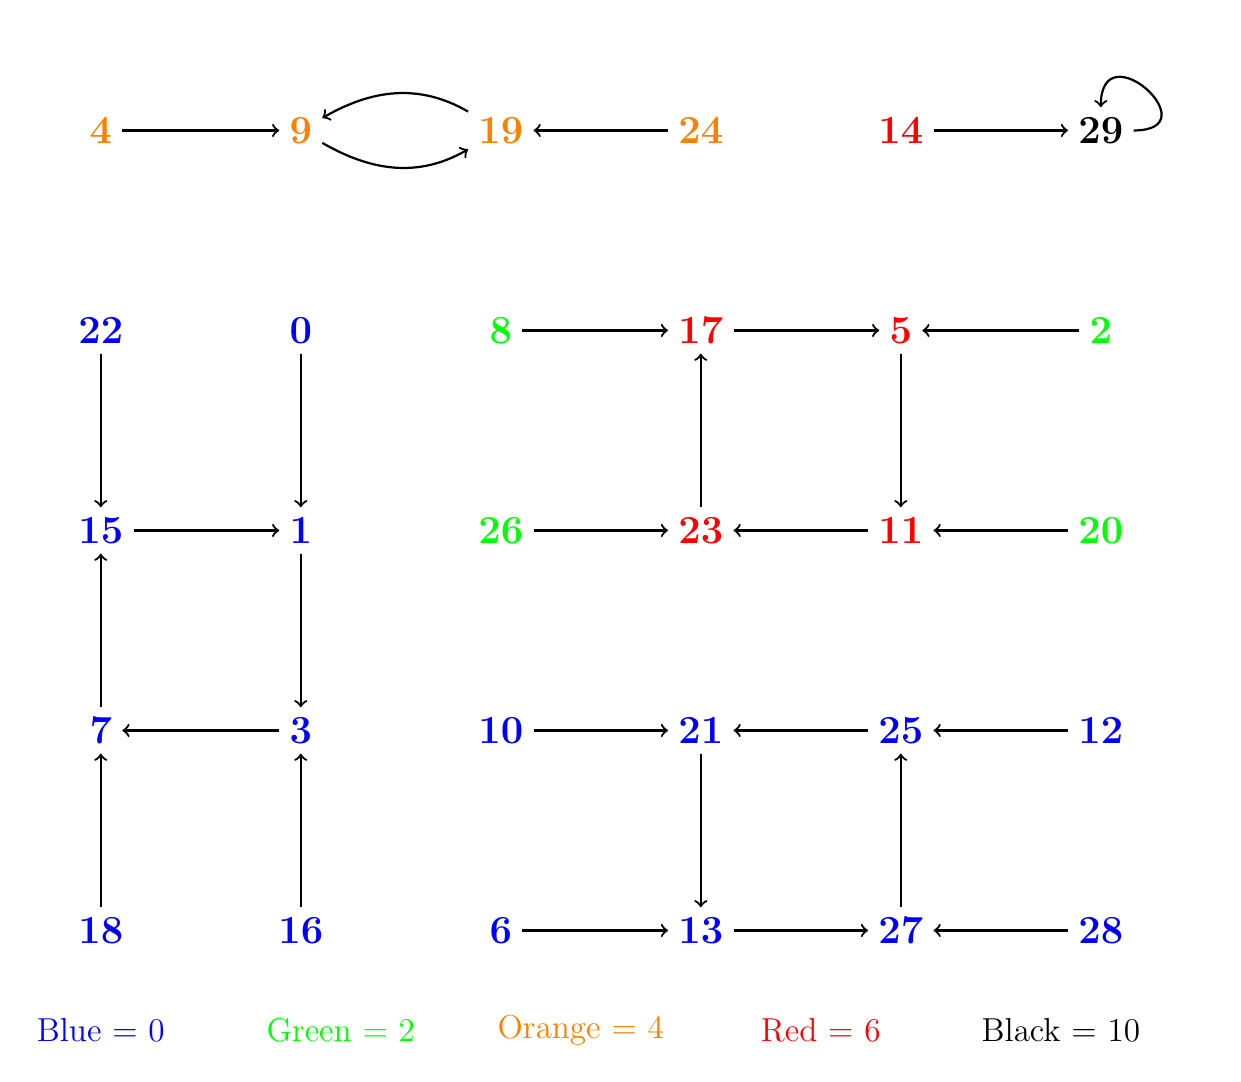
\begin{tikzpicture}
	\node (4) at (0in,4in) [thick, orange] {\Large \bfseries 4};
	\node (9) at (1in,4in) [thick, orange] {\Large \bfseries 9};
	\node (19) at (2in,4in) [thick, orange] {\Large \bfseries 19};
	\node (24) at (3in,4in) [thick, orange] {\Large \bfseries 24};
	\draw[thick, ->] (4) to (9);
	\draw[thick, ->, looseness=1, out=-30, in=-150] (9) to (19);
	\draw[thick, ->, looseness=1, out=150, in=30] (19) to (9);
	\draw[thick, ->] (24) to (19);
	
	\node (14) at (4in,4in) [thick, red] {\Large \bfseries 14};
	\node (29) at (5in,4in) [thick, black] {\Large \bfseries 29};
	\draw[thick, ->] (14) to (29);
	\draw[thick, ->, looseness=5, out=0, in=90] (29) to (29);
	
	\node (22) at (0in,3in) [thick, blue] {\Large \bfseries 22};
	\node (0) at (1in,3in) [thick, blue] {\Large \bfseries 0};
	\node (7) at (0in,1in) [thick, blue] {\Large \bfseries 7};
	\node (3) at (1in,1in) [thick, blue] {\Large \bfseries 3};
	\node (15) at (0in,2in) [thick, blue] {\Large \bfseries 15};
	\node (1) at (1in,2in) [thick, blue] {\Large \bfseries 1};
	\node (18) at (0in,0in) [thick, blue] {\Large \bfseries 18};
	\node (16) at (1in,0in) [thick, blue] {\Large \bfseries 16};
	\draw[thick, ->] (22) to (15);
	\draw[thick, ->] (15) to (1);
	\draw[thick, ->] (1) to (3);
	\draw[thick, ->] (3) to (7);
	\draw[thick, ->] (7) to (15);
	\draw[thick, ->] (0) to (1);
	\draw[thick, ->] (18) to (7);
	\draw[thick, ->] (16) to (3);
	
	\node (8) at (2in,3in) [thick, green] {\Large \bfseries 8};
	\node (17) at (3in,3in) [thick, red] {\Large \bfseries 17};
	\node (26) at (2in,2in) [thick, green] {\Large \bfseries 26};
	\node (23) at (3in,2in) [thick, red] {\Large \bfseries 23};
	\node (5) at (4in,3in) [thick, red] {\Large \bfseries 5};
	\node (2) at (5in,3in) [thick, green] {\Large \bfseries 2};
	\node (11) at (4in,2in) [thick, red] {\Large \bfseries 11};
	\node (20) at (5in,2in) [thick, green] {\Large \bfseries 20};
	\draw[thick, ->] (8) to (17);
	\draw[thick, ->] (17) to (5);
	\draw[thick, ->] (5) to (11);
	\draw[thick, ->] (11) to (23);
	\draw[thick, ->] (23) to (17);
	\draw[thick, ->] (26) to (23);
	\draw[thick, ->] (2) to (5);
	\draw[thick, ->] (20) to (11);
	
	\node (10) at (2in,1in) [thick, blue] {\Large \bfseries 10};
	\node (21) at (3in,1in) [thick, blue] {\Large \bfseries 21};
	\node (25) at (4in,1in) [thick, blue] {\Large \bfseries 25};
	\node (12) at (5in,1in) [thick, blue] {\Large \bfseries 12};	
	\node (6) at (2in,0in) [thick, blue] {\Large \bfseries 6};
	\node (13) at (3in,0in) [thick, blue] {\Large \bfseries 13};
	\node (27) at (4in,0in) [thick, blue] {\Large \bfseries 27};
	\node (28) at (5in,0in) [thick, blue] {\Large \bfseries 28};
	\draw[thick, ->] (10) to (21);
	\draw[thick, ->] (21) to (13);
	\draw[thick, ->] (13) to (27);
	\draw[thick, ->] (27) to (25);
	\draw[thick, ->] (25) to (21);
	\draw[thick, ->] (6) to (13);
	\draw[thick, ->] (28) to (27);
	\draw[thick, ->] (12) to (25);
	
	\node (key-blue) at (0in,-0.5in) [blue] {\large Blue = 0};
	\node (key-green) at (1.2in,-0.5in) [green] {\large Green = 2};
	\node (key-orange) at (2.4in, -0.5in)[orange] {\large Orange = 4}; 
	\node (key-red) at (3.6in, -0.5in) [red] {\large Red = 6};
	\node (key-black) at (4.8in, -0.5in) [black] {\large Black = 10};
	\end{tikzpicture}
	
	I think that corollaries \ref{cor:eigspacedim2n+1}, \ref{cor:0to0},
	\ref{cor:2to6}, \ref{cor:4to4}. \ref{cor:6to6}, \ref{cor:6to10}, and
	\ref{cor:10to10} prove, or at the very least contribute to finding a solution
	for Sutner's conjecture in
	\href{https://drive.google.com/open?id=1b7mSpPkASXAFlvrFL6rWC7dB7qN_-VWf}{\textit{Linear
			Cellular Automata and the Garden of Eden}}.
	We may still need a proof of something similar to conjecture
	\ref{conj:convertedeigval} to prove it in $\Z_2$ rather than $\R$. 
	
	\section{Conjectures}
	\begin{conjecture}\label{conj:convertedli}
		There exist $n$ linearly independent eigenvectors in $\R^{n^2}$ with
		eigenvalue $\lambda = k$ whose converted vectors are linearly independent in
		$\Z_2^{n^2}$.
	\end{conjecture}
	\href{http://www.quandt.com/papers/basicmatrixtheorems.pdf}{This} proof seems
	to be relevant, but I don't know if it applies to finite fields like $\Z_2$.
	
	\begin{conjecture}\label{conj:convertedeigval}
		For $M_{n,k}$ the following hold.
		\begin{enumerate}
			\item All eigenvectors with integer eigenvalues are convertible to a vector
			in $\Z_2^{n^2}$
			\item If $\vec{u} \in \R^{n^2}$ is an eigenvector of $M_{n,k}$ with
			eigenvalue $\lambda$,
			then $\vec{u} \mod 2$ is an eigenvector with eigenvalue $\lambda \mod 2$.
		\end{enumerate}
		
	\end{conjecture}
	The first statement is proven by lemma \ref{lem:convert}.
	I haven't had any luck in proving the second statement.
	Below is an example for a small value of $n$ that demonstrates the idea.
	\begin{example}
		For $n=4$, the eigenvalues with multiplicity are
		\begin{equation*}
		\lambda_4 = \left\{2+\sqrt{5}, 1+\sqrt{5}, 1+\sqrt{5}, \sqrt{5},
		2,2,1,1,1,1,0,0,2-\sqrt{5},1-\sqrt{5},1-\sqrt{5},-\sqrt{5}\right\}.
		\end{equation*}
		If an element of $\lambda_4$ is an integer, then there is a corresponding
		eigenvector with all integer components.
		I won't list all 16 eigenvectors here, but I'll give an example of an integer
		and non-integer eigenvalue.
		
		Take the eigenvalue $\lambda=2$.
		One of the two corresponding eigenvectors is
		\begin{equation*}
		\vec{v}_{\lambda=2} = \begin{bmatrix}
		0  & 1 & 1 & 0  \\
		-1 & 0 & 0 & -1 \\
		-1 & 0 & 0 & -1 \\
		0  & 1 & 1 & 0
		\end{bmatrix}.
		\end{equation*}
		The components have been reshaped into a grid for space concerns and to
		better illustrate the relationship between these vectors and a \textit{Lights
			Out} board.
		We can see that $\vec{v}_{\lambda=2} \in \Z^{25}$.
		We can also check that
		\begin{equation*}
		\vec{v}_{\lambda=2} \mod 2 \equiv \begin{bmatrix}
		0 & 1 & 1 & 0 \\
		1 & 0 & 0 & 1 \\
		1 & 0 & 0 & 1 \\
		0 & 1 & 1 & 0
		\end{bmatrix} \equiv \vec{v}_{\lambda=0}
		\end{equation*}
		meaning that the converted version of $\vec{v}_{\lambda=2}$ is an eigenvector
		in $\Z_2^{16}$ with eigenvalue $0$.
		
		Take the eigenvalue $\lambda=\sqrt{5}$.
		The only corresponding eigenvector is
		\begin{equation*}
		\vec{v}_{\lambda=\sqrt{5}} = \begin{bmatrix}
		1 & \phi-1 & 1-\phi & -1 \\
		\phi-1 & 2-\phi & \phi-2 & 1-\phi \\
		1-\phi & \phi-2 & 2-\phi & \phi-1 \\
		-1 & 1-\phi & \phi-1 & 1
		\end{bmatrix}
		\end{equation*}
		where $\phi$ is the golden ratio.
		Once again, the vector has been reshaped into a grid.
		We can see that since some components are rational and others irrational,
		that $\vec{v}_{\lambda=\sqrt{5}}$ is not convertible to a vector in $\Z_2^{16}$.
		However, if we go ahead and find $\vec{v}_{\lambda=\sqrt{5}} \mod 2$, we see
		that
		\begin{equation*}
		\vec{v}_{\lambda=\sqrt{5}} \mod 2 \equiv \begin{bmatrix}
		1 & 1-\phi & 1-\phi & 1 \\
		1-\phi & 2-\phi & 2-\phi & 1-\phi \\
		1-\phi & 2-\phi & 2-\phi & 1-\phi \\
		1 & 1-\phi & 1-\phi & 1
		\end{bmatrix} \equiv \vec{v}_{\lambda=2-\sqrt{5}}.
		\end{equation*}
		This hints at a deeper relationship between eigenvectors $\mod 2$ whose
		corresponding eigenvalues sum to $2$ (likely to $2k$ in general), likely
		relating to corollary \ref{cor:sum2k}. 
	\end{example}
	Even if true, this conjecture doesn't always give a way to find a basis for
	all null patterns (kernel of $M_{n,k}$ in $\Z_2^{n^2}$).
	For example, the the nullity of $M_{19,1}$ in $\Z_{2}^{361}$ is 16, which is
	greater than the possible number of eigenvalues other than 1 (we showed it was
	at most 10).
	This should imply that certain irrational eigenvalues give convertible
	eigenvectors.
	
	\begin{conjecture}\label{conj:k1evennullity}
		The nullity of $M_{n,1}$ is always even.
	\end{conjecture}
	I couldn't think of a way to extend this to all $k$.
	We may have already proved this.
	We've already proved that the algebraic multiplicity of $\lambda_{i,j} = 0$ is
	even.
	The concern is that the results don't apply in finite fields like $\Z_2$.
	Since $M_{n,1}$ is real and symmetric, it is always diagonalizable, meaning for
	every eigenvalue, the geometric multiplicity equals the algebraic multiplicity.
	It's shown
	\href{https://www.sciencedirect.com/science/article/pii/S0304397504001823}{here}
	that when working in $\Z_2$, the nullity is the degree of
	$\gcd\left(U_n(\frac{x}{2}), U_n(\frac{x+1}{2})\right)$, where $U_n(x)$ is the
	$n$th Chebyshev polynomial as described in lemma \ref{lem:k1eigvals}.
	\href{https://peterefrancis.com/lights-out-algebra/}{Here} is another site that
	makes this claim and  has done some other relevant mathematical analysis of
	\textit{Lights Out}.
	In question 2.3, it asks about a relationship in $\Z_2$ between what we call
	$M_{n,k}$ and $M_{2n+1,k}$ that we have answered in $\R$.
	
	\begin{conjecture}\label{conj:cos_rationals}
		Let $ 0 < p < q < 1$ be rational numbers.
		Let $-2 < C < 2$ be a non-zero rational number.
		The only solutions to
		\begin{equation*}
		\cos{\left(p\pi\right)} + \cos{\left(q\pi\right)} = C
		\end{equation*}
		are 
		\begin{equation*}
		\left(p,q,C \right) = 
		\left(\frac{1}{3}, \frac{1}{3}, 1 \right), 
		\left(\frac{1}{3}, \frac{1}{2}, \frac{1}{2} \right), 
		\left(\frac{1}{5}, \frac{3}{5}, \frac{1}{2} \right), 
		\left(\frac{2}{3}, \frac{2}{3}, -1 \right), 
		\left(\frac{1}{2}, \frac{2}{3}, -\frac{1}{2} \right), \text{and} 
		\left(\frac{2}{5}, \frac{4}{5}, -\frac{1}{2} \right).
		\end{equation*}
	\end{conjecture}
	I have used the method described in lemma \ref{lem:cos_sum1_nosol} to check
	that if any other such solutions do exist, then the denominator of $C$ will be
	greater than $200$.
	In my discussion with Professor Bell, who proved lemma
	\ref{lem:cos_sum1_nosol}, he wondered if we could use some of the properties
	taken advantage of in his proof to provably show that many values of $C$ cannot
	have a solution.
	If we could bound the denominator of $C$ to something computationally
	reasonable, we could then prove this conjecture by checking the remaining
	denominators.
	Conway and Jones also seem to describe the problem more generally and may have
	even solved something equivalent to or even stronger than this conjecture
	\href{http://matwbn.icm.edu.pl/ksiazki/aa/aa30/aa3033.pdf}{here} as theorem 7.	
\end{document}
